\documentclass[pdflatex,compress,mathserif]{beamer}

%\usetheme[dark,framenumber,totalframenumber]{ElektroITK}
\usetheme[darktitle,framenumber,totalframenumber]{ElektroITK}

\usepackage[utf8]{inputenc}
\usepackage[T1]{fontenc}
\usepackage{lmodern}
\usepackage[bahasai]{babel}
\usepackage{amsmath}
\usepackage{amsfonts}
\usepackage{amssymb}
\usepackage{graphicx}
\usepackage{multicol}
\setbeamertemplate{caption}[numbered]

\newcommand*{\Scale}[2][4]{\scalebox{#1}{$#2$}}%

\title{MATRIKULASI}
\subtitle{MATEMATIKA DASAR}

\author{Mifta Nur Farid}

\begin{document}

\maketitle

\section{Pengantar}

	\subsection{Pokok Bahasan}
		\begin{frame}{Pokok Bahasan}
			\begin{multicols}{2}
				\begin{enumerate}
					\item Pertidaksamaan Linier
					\begin{itemize}
						\item Interval
						\item Penyelesaian Pertidaksamaan
					\end{itemize}
					\item Fungsi dan Limit
					\begin{itemize}
						\item Fungsi
						\item Limit
					\end{itemize}
					\item Trigonometri
					\item Turunan
					\item Integral
					\begin{itemize}
						\item Integral Tak Tentu
						\item Integral dengan Substitusi
						\item Integral Tentu
					\end{itemize}
				\end{enumerate}
			\end{multicols}
		\end{frame}

\section{Pertidaksamaan Linier}

	\subsection{Interval}

		\begin{frame}
			\frametitle{Pertidaksamaan}
			\begin{itemize}
				\item Pertidaksamaan:
				\begin{equation}
					5x - 4 > 2x + 3
				\end{equation}
				\item Persamaan menggunakan simbol $ = $
				\item Pertidaksamaan menggunakan simbol
				\begin{center}
					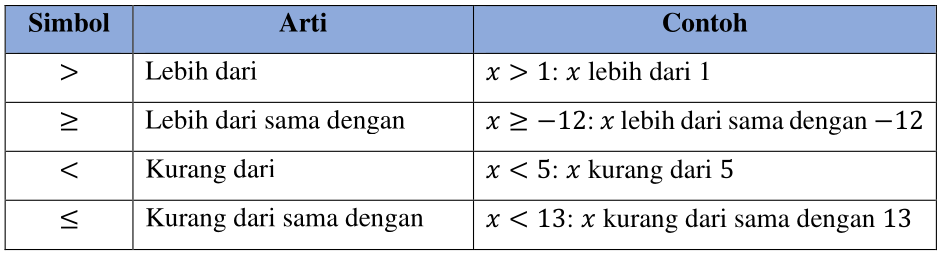
\includegraphics[width=\linewidth]{pict/01}
				\end{center}
			\end{itemize}
		\end{frame}
	
		\begin{frame}{Pertidaksamaan}
			\begin{itemize}
				\item Penyelesaian persamaan
				\begin{align*}
					5x - 4 &= 2x + 3\\
					5x - 2x &= 3 + 4\\
					3x &= 7\\
					x &= \frac{7}{3}
				\end{align*}
				\item Penyelesaian pertidaksamaan: rentang atau nilai variabel yang tidak diketahui yang memenuhi pertidaksamaan
			\end{itemize}
		\end{frame}
	
		\begin{frame}{Interval}
			\begin{itemize}
				\item Himpunan penyelesaian suatu pertidaksamaan dinyatakan dalam notasi himpunan atau bentuk selang atau \textit{interval}
				\item Jenis-jenis selang
				\begin{enumerate}
					\item Selang berhingga dan tertutup
					\item Selang berhingga dan terbuka
					\item Selang berhingga dan setengah terbuka atau setengah tertutup
					\item Selang tak hingga dan tertutup
					\item Selang tak hingga dan terbuka
					\item Selang tak hingga, terbuka, dan tertutup
				\end{enumerate}
			\end{itemize}
		\end{frame}
	
		\begin{frame}
			\frametitle{Selang berhingga dan tertutup}
			\begin{itemize}
				\item Notasi: $ [a,b] $
				\item Dinyatakan dalam notasi himpunan:
				\begin{equation}
					\{x:a \leq x \leq b\}
				\end{equation}
				\item Grafik selang:
				\begin{figure}
					\centering
					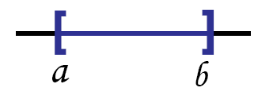
\includegraphics[width=0.5\linewidth]{pict/02}
					\caption{Grafik selang $[a,b]$}
					\label{fig:02}
				\end{figure}
			\end{itemize}
		\end{frame}
	
		\begin{frame}
			\frametitle{Selang berhingga dan terbuka}
			\begin{itemize}
				\item Notasi: $ (a,b) $
				\item Dinyatakan dalam notasi himpunan:
				\begin{equation}
					\{x:a < x < b\}
				\end{equation}
				\item Grafik selang:
				\begin{figure}
					\centering
					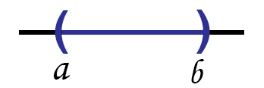
\includegraphics[width=0.5\linewidth]{pict/03}
					\caption{Grafik selang $(a,b)$}
					\label{fig:03}
				\end{figure}
			\end{itemize}
		\end{frame}
	
		\begin{frame}
			\frametitle{Selang berhingga dan setengah terbuka atau setengah tertutup}
			\begin{itemize}
				\item Notasi: $ (a,b] $ atau $ [a,b) $
				\item Notasi himpunan:
				\begin{align*}
					\text{Jika notasi } (a,b] & \text{, maka notasi himpunan }\{x:a < x \leq b\} \\
					\text{Jika notasi } [a,b) & \text{, maka notasi himpunan }\{x:a \leq x < b\} \\
				\end{align*}
				\item Grafik selang:
				\begin{multicols}{2}
					\begin{figure}
						\centering
						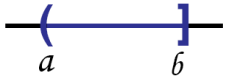
\includegraphics[width=0.5\linewidth]{pict/04}
						\caption{Grafik selang $(a,b]$}
						\label{fig:04}
					\end{figure}
					\columnbreak
					\begin{figure}
						\centering
						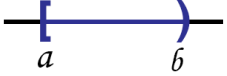
\includegraphics[width=0.5\linewidth]{pict/05}
						\caption{Grafik selang $[a,b)$}
						\label{fig:05}
					\end{figure}
				\end{multicols}
			\end{itemize}
		\end{frame}
		
		\begin{frame}
			\frametitle{Selang tak hingga dan tertutup}
			\begin{itemize}
				\item Notasi: $ [a,+\infty) $ atau $ (-\infty,b] $
				\item Notasi himpunan:
				\begin{align*}
					\text{Jika notasi } [a,+\infty) & \text{, maka notasi himpunan }\{x:x \geq a\} \\
					\text{Jika notasi } (-\infty,b] & \text{, maka notasi himpunan }\{x: x \leq b\} \\
				\end{align*}
				\item Grafik selang:
				\begin{multicols}{2}
					\begin{figure}
						\centering
						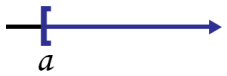
\includegraphics[width=0.5\linewidth]{pict/06}
						\caption{Grafik selang $[a,+\infty)$}
						\label{fig:06}
					\end{figure}
					\columnbreak
					\begin{figure}
						\centering
						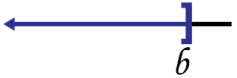
\includegraphics[width=0.5\linewidth]{pict/07}
						\caption{Grafik selang $(-\infty,b]$}
						\label{fig:07}
					\end{figure}
				\end{multicols}
			\end{itemize}
		\end{frame}
	
		\begin{frame}
			\frametitle{Selang tak hingga dan terbuka}
			\begin{itemize}
				\item Notasi: $ (a,+\infty) $ atau $ (-\infty,b) $
				\item Notasi himpunan:
				\begin{align*}
					\text{Jika notasi } (a,+\infty) & \text{, maka notasi himpunan }\{x:x > a\} \\
					\text{Jika notasi } (-\infty,b) & \text{, maka notasi himpunan }\{x: x < b\} \\
				\end{align*}
				\item Grafik selang:
				\begin{multicols}{2}
					\begin{figure}
						\centering
						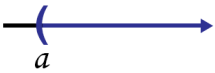
\includegraphics[width=0.5\linewidth]{pict/08}
						\caption{Grafik selang $(a,+\infty)$}
						\label{fig:08}
					\end{figure}
					\columnbreak
					\begin{figure}
						\centering
						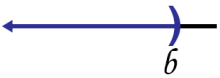
\includegraphics[width=0.5\linewidth]{pict/09}
						\caption{Grafik selang $(-\infty,b)$}
						\label{fig:09}
					\end{figure}
				\end{multicols}
			\end{itemize}
		\end{frame}
		
		\begin{frame}
			\frametitle{Selang tak hingga}
			\begin{itemize}
				\item Notasi: $ (-\infty,+\infty) $
				\item Notasi himpunan:
				\begin{equation*}
					\{ x : x \in \mathcal{R} \}
				\end{equation*}
				\item Grafik selang:
				\begin{figure}
					\centering
					
\includegraphics[width=0.5\linewidth]{pict/10}
					\caption{Grafik selang $(-\infty,+\infty)$}
					\label{fig:10}
				\end{figure}
			\end{itemize}
		\end{frame}
	
	\subsection{Penyelesaian Pertidaksamaan}
	
		\begin{frame}
			\frametitle{Penyelesaian pertidaksamaan}
			Hal-hal yang perlu diperhatikan dalam menyelesaikan suatu pertidaksamaan
			\begin{enumerate}
				\item Prosedur menyelesaikan pertidaksamaan adalah mengubah pertidaksamaan satu langkah demi satu langkah hingga diperoleh himpunan penyelesaiannya jelas.
				\item Dapat dilakukan operasi-operasi tertentu (tambah, kurang, kali, bagi, akar, pangkat) pada kedua ruas pada suatu pertidaksamaan. Perlakuan pada kedua ruas harus sama, contohnya:
				\begin{enumerate}
					\item Kedua ruas ditambah atau dikurangi dengan suatu bilangan;
					\item Kedua ruas dikali atau dibagi dengan suatu bilangan positif;
					\item Jika kedua ruas dikali atau dibagi dengan bilangan negatif, tanda pertidaksamaan harus berbalik arah.
				\end{enumerate}
			\end{enumerate}
		\end{frame}
	
	\subsection{Contoh Soal}
	
		\begin{frame}
			\frametitle{Contoh 1}
			Selesaikan pertidaksamaan
			\begin{equation*}
				-5x - 10 < 15
			\end{equation*}
			dan tunjukkan garis bilangan himpunan penyelesaiannya.
		\end{frame}
	
		\begin{frame}
			\frametitle{Jawaban Contoh 1}
			\begin{align*}
				-5x - 10 & < 15 &\\
				-5x - 10 + 10 & < 15 + 10 & \text{(kedua ruas ditambah 10)} \\
				-5x & < 25 & \\
				\frac{-5x}{-5} & > \frac{25}{-5} & \text{(kedua ruas dikali dengan } -\frac{1}{5} \text{)}\\
				x & > -5
			\end{align*}
		\end{frame}
		
		\begin{frame}{Jawaban Contoh 1}
			\begin{itemize}
				\item Himpunan penyelesaiannya adalah $ \{ x : x > -5 \} $, atau \item Dalam bentuk selang $ (-5,+\infty) $.
				\item Berikut $ (-5,+\infty) $ diinterpretasikan dalam bentuk garis bilangan.
				\begin{figure}
					\centering
					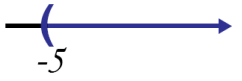
\includegraphics[width=0.3\linewidth]{pict/11}
					\caption{Grafik selang $(-5,+\infty)$}
					\label{fig:11}
				\end{figure}
			\end{itemize}
		\end{frame}
		
		\begin{frame}
			\frametitle{Contoh 2}
			Selesaikan pertidaksamaan
			\begin{equation*}
				-5 \leq 2x + 6 < 4
			\end{equation*}
			dan tunjukkan garis bilangan himpunan penyelesaiannya.
		\end{frame}
	
		\begin{frame}
			\frametitle{Jawaban Contoh 2}
			\begin{tabular}{rcccll}
				$ -5 $ & $\leq$ & $ 2x + 6 $ & < & $ 4 $ &  \\
				$ -5-6 $ & $\leq$ & $ 2x + 6 - 6 $ & < & $ 4 - 6 $ & (dikurangin 6) \\
				$ -11 $ & $\leq$ & $ 2x $ & < & $ -2 $ & \\
				$-11/2$ & $\leq$ & $2x/2$ & < & $-2/2$ & (dibagi 2 atau dikali $\frac{1}{2}$)\\
				$ -11/2 $ & $\leq$ & $ x $ & < & $ -1 $ &  \\
			\end{tabular}
		\end{frame}
		
		\begin{frame}{Jawaban Contoh 2}
			Himpunan penyelesaiannya adalah
			\begin{equation*}
				\left\{ x:-\frac{11}{2} \leq x < -1 \right\}
			\end{equation*}
			atau ditulis dalam bentuk selang $ \left[ -\frac{11}{2}, -1 \right) $ atau dengan garis bilangan
			\begin{figure}
				\centering
				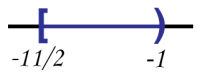
\includegraphics[width=0.3\linewidth]{pict/12}
				\caption{Grafik selang $ \left[ -\frac{11}{2}, -1 \right) $ }
				\label{fig:12}
			\end{figure}
		\end{frame}
		
		\begin{frame}
			\frametitle{Contoh 3}
			Selesaikan pertidaksamaan 
			\begin{equation*}
				x^2 - x < 6
			\end{equation*}
		\end{frame}
	
		\begin{frame}
			\frametitle{Jawaban Contoh 3}
			\begin{align*}
				x^2 - x &< 6 &\\
				x^2 - x - 6 & < 6 - 6 & \text{(dikurangi 6)}\\
				(x+2)(x-3)& <  0 &\text{(difaktorkan)}\\
			\end{align*}
			\begin{itemize}
				\item Dapat dilihat bahwa $ x = -2 $ dan $ x = 3 $ membagi garis bilangan kedalam tiga selang terbuka yaitu $ (-\infty, -2) $, $ (-2,3) $, dan $ (3, +\infty) $.
				\item Selanjutnya kita harus mengecek setiap tanda diselang dengan cara diambil satu titik yang berada di tiga selang tersebut.
			\end{itemize}
		\end{frame}
	
		\begin{frame}{Jawaban Contoh 3}
			\begin{itemize}
				\item $ x = -3 $ mewakili titik yang berada pada selang $ (-\infty, -2) $
				\item $ x = 0 $ mewakili titik yang berada pada selang $ (-2, 3) $
				\item $ x = 5 $ mewakili titik yang berada pada selang $ (3, +\infty) $
				\begin{figure}
					\centering
					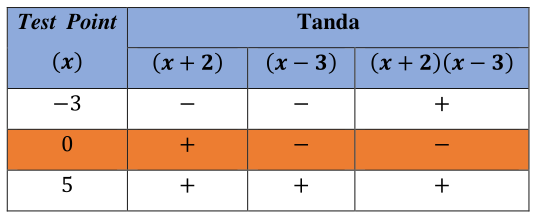
\includegraphics[width=0.7\linewidth]{pict/13}
				\end{figure}
				\item Daerah yang memenuhi $ (x+2)(x-3)<0 $ adalah selang $ (-2,3) $
			\end{itemize}
			
		\end{frame}
	
		\begin{frame}{Jawaban Contoh 3}
			Himpunan penyelesaiannya adalah
			$$ \{x: -2 < x < 3\} $$
			atau dalam bentuk selang $ (-2,3) $ atau dengan garis bilangan
			\begin{figure}
				\centering
				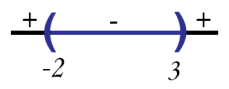
\includegraphics[width=0.3\linewidth]{pict/14}
				\caption{Grafik selang $ (-2,3) $ dan tanda di masing-masing daerahnya}
				\label{fig:14}
			\end{figure}
		\end{frame}
	
		\begin{frame}
			\frametitle{Contoh 4}
			Selesaikan pertidaksamaan
			\begin{equation*}
				3x^2 - x - 2 \geq 0
			\end{equation*}
		\end{frame}
	
		\begin{frame}
			\frametitle{Jawaban Contoh 4}
			\begin{align*}
				3x^2 - x - 2 &\geq 0 &\\
				(x-1)(3x+2) &\geq 0 & \text{(difaktorkan)}
			\end{align*}
			\begin{itemize}
				\item Dapat dilihat bahwa $ x = -\frac{2}{3}$ dan $ x = 1 $ membagi garis bilangan ke dalam tiga selang tertutup yaitu $ (-\infty, -\frac{2}{3}] $, $ [-\frac{2}{3} , 1] $, dan $ [1, +\infty) $.
			\end{itemize}
		\end{frame}
	
		\begin{frame}{Jawaban Contoh 4}
			\begin{itemize}
				\item Uji tanda
				\begin{figure}
					\centering
					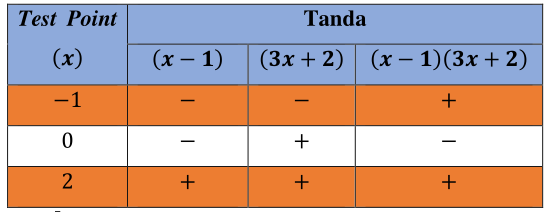
\includegraphics[width=0.7\linewidth]{pict/15}
				\end{figure}
			\end{itemize}
		\end{frame}
	
		\begin{frame}{Jawaban Contoh 4}
			Himpunan penyelesaiannya adalah
			$$ \{x: x \leq -\frac{2}{3} \cup x \geq 1\} $$
			atau dalam bentuk selang $ \left(-\infty,-\frac{2}{3} \right] \cup \left[ 1,+\infty \right) $ atau dengan garis bilangan
			\begin{figure}
				\centering
				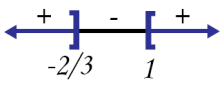
\includegraphics[width=0.3\linewidth]{pict/16}
				\caption{Grafik selang $ \left(-\infty,-\frac{2}{3} \right] \cup \left[ 1,+\infty \right) $ dan tanda di masing-masing daerahnya}
				\label{fig:16}
			\end{figure}
		\end{frame}
	
		\begin{frame}
			\frametitle{Contoh 5}
			Selesaikan pertidaksamaan
			\begin{equation*}
				\frac{x - 1}{x + 2} \geq 0
			\end{equation*}
		\end{frame}
		
		\begin{frame}
			\frametitle{Jawaban Contoh 5}
			\begin{itemize}
				\item Perhatikan masing-masing persamaan yang menjadi pembilang dan penyebut saat sama dengan nol.
				\begin{itemize}
					\item Nilai $ x - 1 = 0 $ jika $ x = 1 $
					\item Nilai $ x + 2 = 0 $ jika $ x = -2 $
				\end{itemize}
				\item $ x = 1 $ dan $ x = -2 $ menghasilkan 3 selang yaitu $ (-\infty,-2) $, $ (-2,1] $, dan $ [1,+\infty) $
				\begin{itemize}
					\item Selang $ (-\infty,-2) $ tidak tertutup di $ x = -2 $ karena apabila disubstitusikan $ x = -2 $ ke persamaan $\frac{x-1}{x+2}$ akan membuat penyebutnya bernilai nol.
				\end{itemize}
				\item Selanjutnya dilakukan uji tanda
			\end{itemize}
		\end{frame}
	
		\begin{frame}{Jawaban Contoh 5}
			\begin{itemize}
				\item Uji tanda
				\begin{figure}
					\centering
					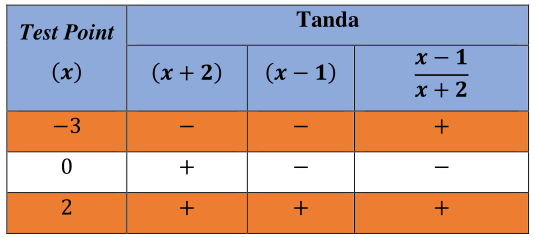
\includegraphics[width=0.7\linewidth]{pict/17}
				\end{figure}
			\end{itemize}
		\end{frame}
		
		\begin{frame}{Jawaban Contoh 5}
			Himpunan penyelesaiannya adalah
			$$ \{x: x \leq -2 \cup x \geq 1\} $$
			atau dalam bentuk selang $ \left(-\infty,-2 \right) \cup \left[ 1,+\infty \right) $ atau dengan garis bilangan
			\begin{figure}
				\centering
				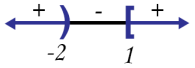
\includegraphics[width=0.3\linewidth]{pict/18}
				\caption{Grafik selang $ \left(-\infty,-2 \right) \cup \left[ 1,+\infty \right) $ dan tanda di masing-masing daerahnya}
				\label{fig:18}
			\end{figure}
		\end{frame}
	
	\subsection{Latihan Soal}
	
	\begin{frame}
		\frametitle{Latihan Soal}
		Selesaikan pertidaksamaan dibawah ini dan sketsakan himpunan penyelesaiannya pada garis koordinat:
		\begin{enumerate}
			\item $ 3x - 5 > -7x -4 $
			\item $ 2(x+3) < x + 1 $
			\item $ 1 \leq 2 - 3x < 8 $
			\item $ 2x^2 + 3x - 2 \leq 0 $
			\item $ \frac{2}{x - 5} \geq \frac{1}{x + 1}$
		\end{enumerate}
	\end{frame}
	
\section{Fungsi Dan Limit}

	\subsection{Fungsi}
	
		\begin{frame}
			\frametitle{Fungsi}
			\begin{itemize}
				\item Sebuah fungsi $ f $ adalah suatu aturan korespondensi yang menghubungkan setiap objek $ x $ dalam satu himpunan yang disebut daerah asal/\textit{domain}, dengan sebuah nilai tunggal $ f(x) $ dari suatu himpunan kedua (kodomain).
				\item Himpunan nilai yang diperoleh dari $ f(x) $ disebut daerah hasil/\textit{range}.
				\item Umumnya, fungsi dinotasikan sebagai $ y = f(x) $ dengan $ x $ adalah peubah (variabel) bebas dari $ f $ yang merupakan domain, sedangkan $ y $ merupakan peubah (variabel) tak bebas dari $ y $.
				\begin{itemize}
					\item Berarti nilai $ y $ yang dihasilkan bergantung pada nilai $ x $ yang diberikan.
				\end{itemize}
				\item Nilai-nilai $ x $ merupakan anggota dari domain fungsi $ f $ dan $ y $ merupakan anggota dari \textit{range} fungsi $ f $.
			\end{itemize}
		\end{frame}
	
		\begin{frame}{Fungsi}
			\begin{itemize}
				\item Jika didefinisikan fungsi $ y = f(x) $, maka domain (daerah asal) dari $ f $ merupakan himpunan nilai – nilai dari himpunan bebas (variabel) $ x $ yang dinotasikan sebagai $ D_f $.
				\item Sedangkan \textit{range} merupakan semua nilai $ f(x) $ untuk setiap $ x $ pada domain $ f $. \textit{Range} dari fungsi $ f $ dinotasikan sebagai $ R_f $ .
			\end{itemize}
		\end{frame}
	
		\begin{frame}{Fungsi}
			\begin{itemize}
				\item Diberikan dua buah fungsi $ f $ dan $ g $, maka rumus-rumus untuk jumlah $ f+g $, selisih $ f-g $, hasil kali $ f \cdot g $, dan hasil bagi $ \frac{f}{g} $ didefinisikan sebagai
				\begin{align*}
					(f+g)(x) &= f(x) + g(x) \\
					(f-g)(x) &= f(x) - g(x) \\
					(f \cdot g)(x) &= f(x) \cdot g(x) \\
					\left( \frac{f}{g} \right)(x) &= \frac{f(x)}{g(x)},~g(x) \neq 0
				\end{align*}
				\item Komposisi fungsi $ f $ dan $ g $ dinyatakan sebagai berikut
				\begin{equation*}
					(f \circ g)(x) = f(g(x))
				\end{equation*}
				atau dinotasikan $ f \circ g $
			\end{itemize}
		\end{frame}
		
		\begin{frame}
			\frametitle{Contoh 1}
			Diberikan suatu fungsi $ f(x) = x^2 - 2x $, tentukan dan sederhanakan nilai dari
			\begin{enumerate}
				\item $ f(x) $
				\item $ f(4+h) $
				\item $\frac{f(4+h) - f(4)}{h}$
			\end{enumerate}
		\end{frame}
	
		\begin{frame}
			\frametitle{Jawaban Contoh 1}
			\begin{enumerate}
				\item $ f(4) = (4)^2 - 2(4) = 8 $
				\item $ f(4+h) = (4+h)^2 - 2(4+h) = 16 + 8h + h^2 - 8 - 2h = 8 + 6h + h^2 $
				\item $\frac{f(4+h) - f(4)}{h} = \frac{8 + 6h + h^2 - 8}{h} = \frac{6h+h^2}{h} = 6 + h$
			\end{enumerate}
		\end{frame}
	
		\begin{frame}
			\frametitle{Contoh 2}
			Selidiki domain dan \textit{range} dari $ g(x) = 1 + \sqrt{x} $
		\end{frame}
	
		\begin{frame}
			\frametitle{Jawaban Contoh 2}
			Domain dari fungsi $ g(x) $ adalah $ [0, +\infty) $. Ketika nilai - nilai pada domain $ [0, +\infty) $ disubstitusikan ke dalam $ 1 + \sqrt{x} $, maka diperoleh range dari $ g $ yaitu $ [1, +\infty) $.
		\end{frame}
		
		\begin{frame}
			\frametitle{Soal Latihan}
			\begin{enumerate}
				\item Diberikan fungsi
				\begin{equation*}
					f(x) = \begin{cases}
						2x^3 - 8,	& \text{ jika } x \leq 3\\
						\sqrt{x-3}, & \text{ jika } x > 3
					\end{cases}
				\end{equation*}
				\begin{enumerate}
					\item $ f(4) $
					\item $ f(\frac{1}{2}) $
					\item $ f(3 - t^2) $
				\end{enumerate}
				\item Selidiki domain dan range dari fungsi - fungsi berikut:
				\begin{enumerate}
					\item $ f(x) = \frac{1}{x} $
					\item $ g(x) = \frac{1}{x^2 + 1} $
					\item $ h(x) = \sqrt{2x - 1}$
					\item $ i(x) = \frac{2}{\sqrt{x^2 - 4}} $
				\end{enumerate}
			\end{enumerate}
		\end{frame}
		
		\begin{frame}{Soal Latihan}
			\begin{enumerate}\setcounter{enumi}{2}
				\item Diberikan fungsi $ f(x) = x- 1 $. Tentukan rumus fungsi dan domain dari:
				\begin{enumerate}
					\item $ f(2x) + f(\sqrt{x}) $
					\item $ f(x^2) - f(-x) $
					\item $ f(1-t) + 2f^2(t) $
				\end{enumerate}
				\item Selidiki komposisi fungsi $ f $ terhadap $ g $ dan domainnya jika diberikan fungsi $ f $ dan $ g $ sebagai berikut:
				\begin{enumerate}
					\item $ f(x) = \sqrt{x} \text{ dan } g(x) = \frac{1}{x}$
					\item $ f(x) = x^2 + x - 1 \text{ dan } g(x) = 1 - \sqrt{x} $
				\end{enumerate}
			\end{enumerate}
		\end{frame}
	
	\subsection{Limit}
	
		\begin{frame}
			\frametitle{Limit}
			\begin{itemize}
				\item Limit fungsi adalah perilaku suatu fungsi mendekati suatu nilai tertentu.
				\item Limit terbagi menjadi dua yaitu limit kiri dan limit kanan dari suatu fungsi.
				\item Limit kiri dari suatu fungsi $ f(x) $ mendekati suatu nilai $ x_0 $ dinotasikan sebagai
				\begin{equation*}
					\lim\limits_{x \rightarrow x_0^-}f(x)
				\end{equation*}
				\item Limit kanan dari suatu fungsi $ f(x) $ mendekati suatu nilai $ x_0 $ dinotasikan sebagai
				\begin{equation*}
					\lim\limits_{x \rightarrow x_0^+}f(x)
				\end{equation*}
			\end{itemize}
		\end{frame}
	
		\begin{frame}{Limit}
			\begin{itemize}
				\item Limit dua sisi dari suatu fungsi $ f(x) $ dinotasikan dengan
				\begin{equation*}
					\lim\limits_{x \rightarrow x_0}f(x) = L
				\end{equation*}
				\item Jika nilai dari limit kanan dan limit kiri dari suatu fungsi $ f $ sama, maka dapat disimpulkan bahwa fungsi $ f $ memiliki limit dan nilai limitnya adalah $ L $.
				\item \textbf{Perlu diperhatikan dalam mengerjakan soal limit, nilai fungsi $ f(x) $ harus terdefinisi di $ x = x_0 $ atau $ \lim\limits_{x \rightarrow x_0} f(x) \neq \frac{0}{0} $ }
				\item Apabila bertemu dengan fungsi yang seperti ini, maka fungsi $ f(x) $ harus diserderhanakan terlebih dahulu untuk mendapatkan nilai limitnya. Salah satu caranya adalah dengan
				pemfaktoran.
			\end{itemize}
		\end{frame}
	
		\begin{frame}{Limit}
			Aturan dasar limit meliputi
			\begin{align*}
				\lim\limits_{x \rightarrow c} k &= k \\
				\lim\limits_{x \rightarrow - \infty} k &= k \\
				\lim\limits_{x \rightarrow + \infty} k &= k \\
				\lim\limits_{x \rightarrow c} x &= c \\
				\lim\limits_{x \rightarrow - \infty} x &= - \infty \\
				\lim\limits_{x \rightarrow + \infty} x &= + \infty \\
			\end{align*}
			dengan $ k $ dan $ c $ konstanta.
		\end{frame}
	
		\begin{frame}{Limit}
			Jika didefinisikan dua buah fungsi, $ f $ dan $ g $ yang memiliki limit masing-masing, yaitu $ L_1 $ dan $ L_2 $ maka:
			\begin{itemize}
				\item[$\bullet$] $ \lim[f(x) + g(x)] = \lim f(x) + \lim g(x) = L_1 + L_2 $
				\item[$\bullet$] $ \lim[f(x) - g(x)] = \lim f(x) - \lim g(x) = L_1 - L_2 $
				\item[$\bullet$] $ \lim[f(x)g(x)] = \lim f(x) \cdot \lim g(x) = L_1L_2 $
				\item[$\bullet$] $ \lim\left[\frac{f(x)}{g(x)}\right] = \frac{\lim f(x)}{\lim g(x)} = \frac{L_1}{L_2},~\text{ jika } L_2 \neq 0 $
				\item[$\bullet$] $ \lim \sqrt[n]{f(x)} = \sqrt[n]{\lim f(x)} = \sqrt[n]{ L_1 }$ untuk $ L_1 \geq 0 $ jika $ n $ genap
				\item[$\bullet$] $ \lim \left[ f(x) \right] ^n = \left[ \lim f(x) \right]^n $
				\item[$\bullet$] $ \lim k f(x) = \lim k \cdot \lim f(x) = k \cdot \lim f(x) $
			\end{itemize}
			Notasi $ \lim $ dapat menyatakan $ \lim\limits_{x \rightarrow c} $, $ \lim\limits_{x \rightarrow c^-} $, $ \lim\limits_{x \rightarrow c^+} $, $ \lim\limits_{x \rightarrow - \infty} $, dan $ \lim\limits_{x \rightarrow + \infty} $
		\end{frame}
	
		\begin{frame}
			\frametitle{Contoh 3}
			Tentukan
			\begin{equation*}
				\lim\limits_{x \rightarrow 2} \left( x^3 - 2\sqrt{x} - 3 \right)
			\end{equation*}
		\end{frame}

		\begin{frame}
			\frametitle{Jawaban Contoh 3}
			\begin{align*}
				\lim\limits_{x \rightarrow 2} \left( x^3 - 2\sqrt{x} - 3 \right) & = \lim\limits_{x \rightarrow 2} x^3 - \lim\limits_{x \rightarrow 2} 2\sqrt{x} - \lim\limits_{x \rightarrow 2} 3 \\
				& = \left[\lim\limits_{x \rightarrow 2} x^3\right] - 2\lim\limits_{x \rightarrow 2} \sqrt{x} - \lim\limits_{x \rightarrow 2} 3 \\
				& = \left[\lim\limits_{x \rightarrow 2} x^3\right] - 2\sqrt{\lim\limits_{x \rightarrow 2} x} - \lim\limits_{x \rightarrow 2} 3 \\
				& = [2]^3 - 2\sqrt{2} - 3 \\
				& = 5 - 2\sqrt{2}
			\end{align*}
		\end{frame}
	
		\begin{frame}
			\frametitle{Contoh 4}
			Tentukan
			\begin{equation*}
				\lim\limits_{x \rightarrow 3} \left( \frac{x^2 - 5x + 6}{x - 3} \right)
			\end{equation*}
		\end{frame}
	
		\begin{frame}
			\frametitle{Jawaban Contoh 4}
			Dalam dilihat bahwa $ \lim\limits_{x \rightarrow 3} \left( \frac{x^2 - 5x + 6}{x - 3} \right) = \frac{0}{0} $. Oleh karena itu, fungsi rasional tersebut harus disederhanakan dengan metode pemfaktoran untuk mengetahui nilai limitnya
			\begin{align*}
				\lim\limits_{x \rightarrow 3} \left( \frac{x^2 - 5x + 6}{x - 3} \right) &= \lim\limits_{x \rightarrow 3} \left( \frac{(x-3)(x-2)}{x - 3} \right) \\
				&= \lim\limits_{x \rightarrow 3} \left( x-2\right) \\
				&= 3 - 2 \\
				&= 1
			\end{align*}
		\end{frame}

		\begin{frame}
			\frametitle{Soal Latihan}
			\begin{enumerate}
				\item Tentukan nilai limit dari:
				\begin{enumerate}
					\item $\lim\limits_{x \rightarrow 3} \left( x^2 - 20 \right)$
					\item $\lim\limits_{x \rightarrow -1} \left( 4x^2 + 3x + 1 \right)$
					\item $\lim\limits_{x \rightarrow -2} \left( \frac{x^2 - 2x - 8}{x^2 - 4} \right)$
					\item $\lim\limits_{x \rightarrow 2} \left( \frac{x^2 - 4}{3 - \sqrt{x^2+5}} \right)$
					\item $\lim\limits_{x \rightarrow 2} \left( \frac{3 - \sqrt{x+7}}{x^2 + x - 6} \right)$
				\end{enumerate}
				\item Diketahui $ f(x) = \begin{cases}
					x^2;	& x \leq 0 \\
					x, 		& 0 < x \leq 1 \\
					1 + x,	& x > 1
				\end{cases} $,
				tentukan apakah $ \lim\limits_{x \rightarrow 0} f(x) $ dan $ \lim\limits_{x \rightarrow 1} f(x) $ (jika ada)!
			\end{enumerate}
		\end{frame}
	
\section{Trigonometri}

	\begin{frame}
		\frametitle{Trigonometri}
		\begin{itemize}
			\item Trigonometri berasal dari bahasa Yunani.
			\item Trigonometri berasal dari dua kata, yaitu \textit{trigono} berarti segitiga dan \textit{metri} berarti ilmu ukur.
			\item Trigonometri adalah ilmu matematika yang mempelajari tentang segitiga siku-siku.
			\item Pada segitiga siku-siku berlaku teorema Phytagoras dan nilai perbandingan sisi-sisi segitiga siku-siku.
			\item Nilai perbandingan trigonometri adalah nilai perbandingan sisi-sisi segitiga siku-siku.
		\end{itemize}
	\end{frame}

	\begin{frame}{Trigonometri}
		\begin{itemize}
			\item Macam definisi dari nilai perbandingan trigonometri:
			\begin{center}
				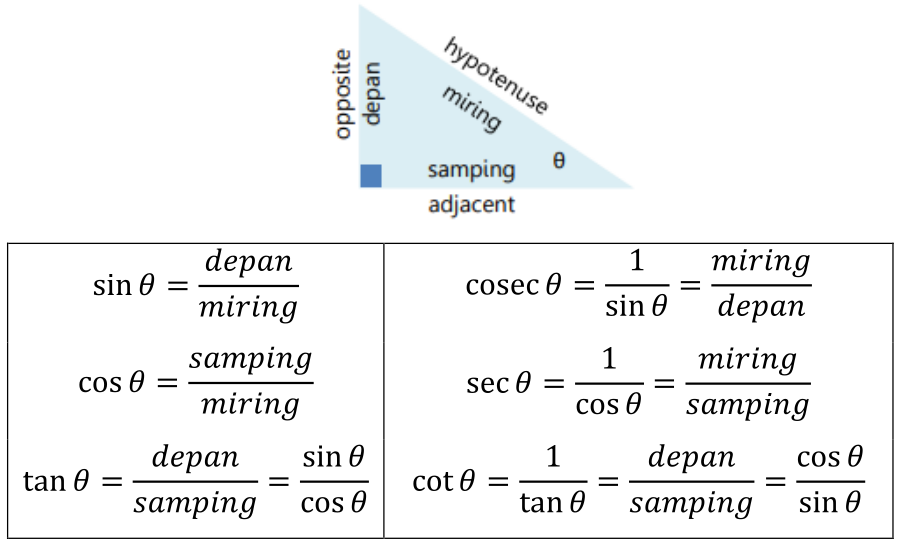
\includegraphics[width=0.8\linewidth]{pict/19}
			\end{center}
		\end{itemize}
	\end{frame}

	\begin{frame}{Trigonometri}
		\begin{itemize}
			\item Perbandingan nilai sisi-sisi segitiga istimewa dan sudutnya antara lain:
			\begin{center}
				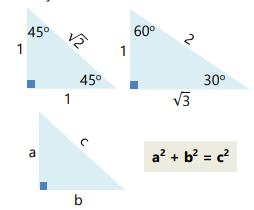
\includegraphics[width=0.6\linewidth]{pict/20}
			\end{center}
		\end{itemize}
	\end{frame}
	
	\begin{frame}{Trigonometri}
		\begin{itemize}
			\item Nilai perbandingan trigonometri pada sudutsudut istimewa:
			\begin{center}
				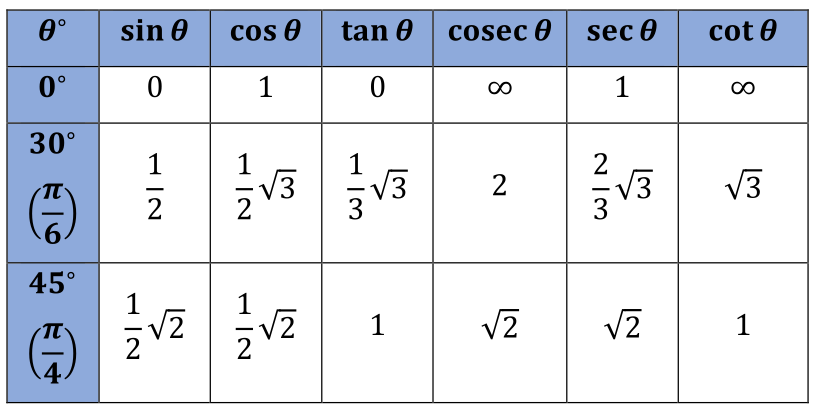
\includegraphics[width=0.7\linewidth]{pict/21}
				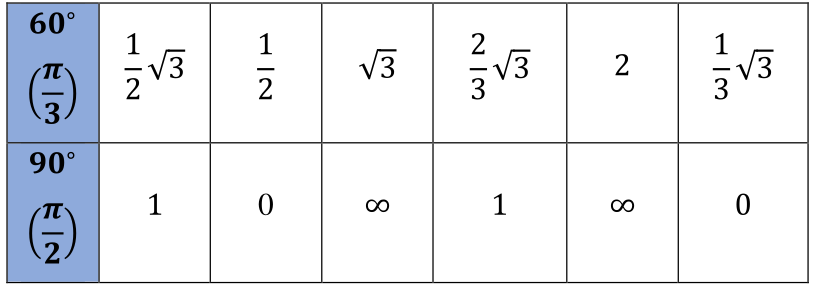
\includegraphics[width=0.7\linewidth]{pict/22}
			\end{center}
		\end{itemize}
	\end{frame}
	
	\begin{frame}{Trigonometri}
		\begin{itemize}
			\item Nilai perbandingan trigonometri suatu sudut yang besarnya $ < 90^{\circ} $ dapat dijelaskan melalui kuadran koordinat kartesius.
			\begin{center}
				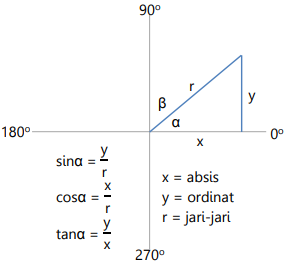
\includegraphics[width=0.5\linewidth]{pict/23}
			\end{center}
		\end{itemize}
	\end{frame}

	\begin{frame}{Trigonometri}
		\begin{itemize}
			\item Tanda nilai perbandingan trigonometri berbeda di masing-masing kuadrannya.
			\begin{center}
				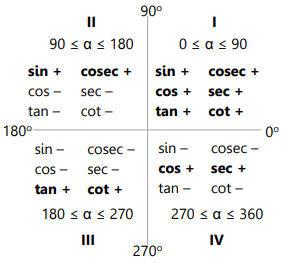
\includegraphics[width=0.5\linewidth]{pict/24}
			\end{center}
		\end{itemize}
	\end{frame}

	\begin{frame}{Trigonometri}
		\begin{itemize}
			\item Perbandingan trigonometri sudut berelasi sebagai berikut
			\begin{center}
				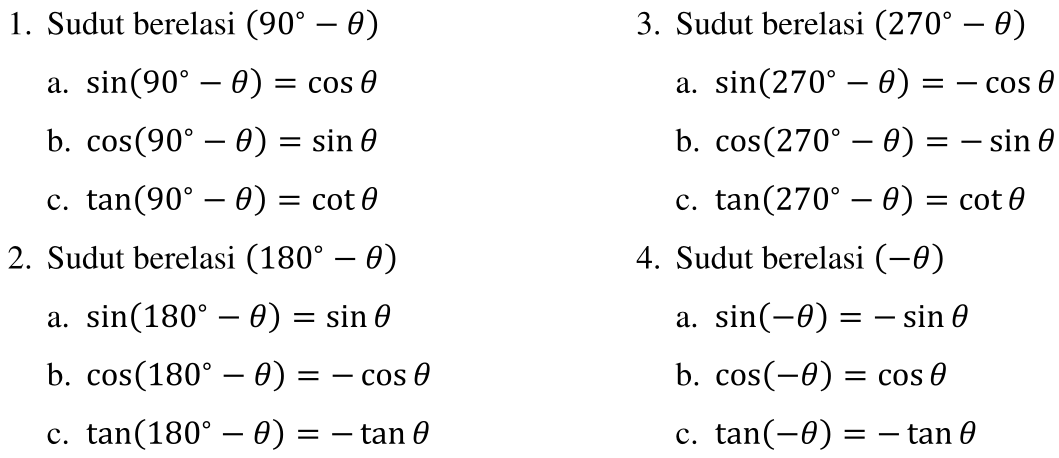
\includegraphics[width=\linewidth]{pict/25}
			\end{center}
		\end{itemize}
	\end{frame}

	\begin{frame}{Trigonometri}
		\begin{center}
			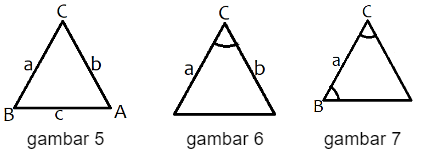
\includegraphics[width=0.5\linewidth]{pict/26}
			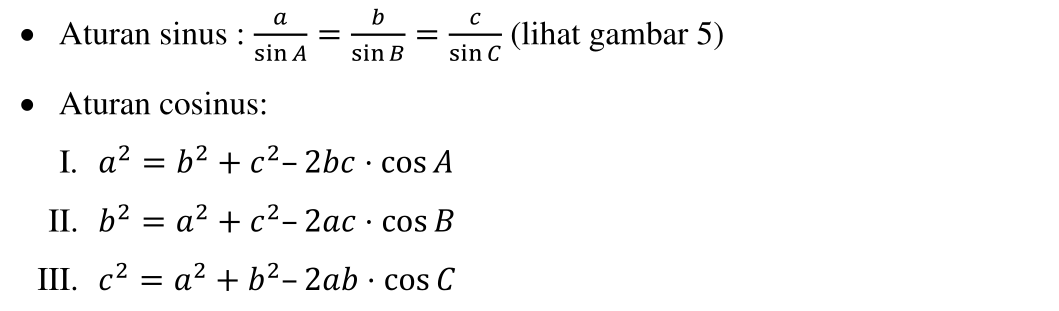
\includegraphics[width=0.9\linewidth]{pict/27}
		\end{center}
	\end{frame}
	
	\begin{frame}{Trigonometri}
		\begin{center}
			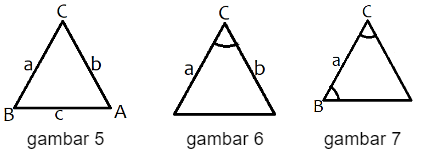
\includegraphics[width=0.5\linewidth]{pict/26}
			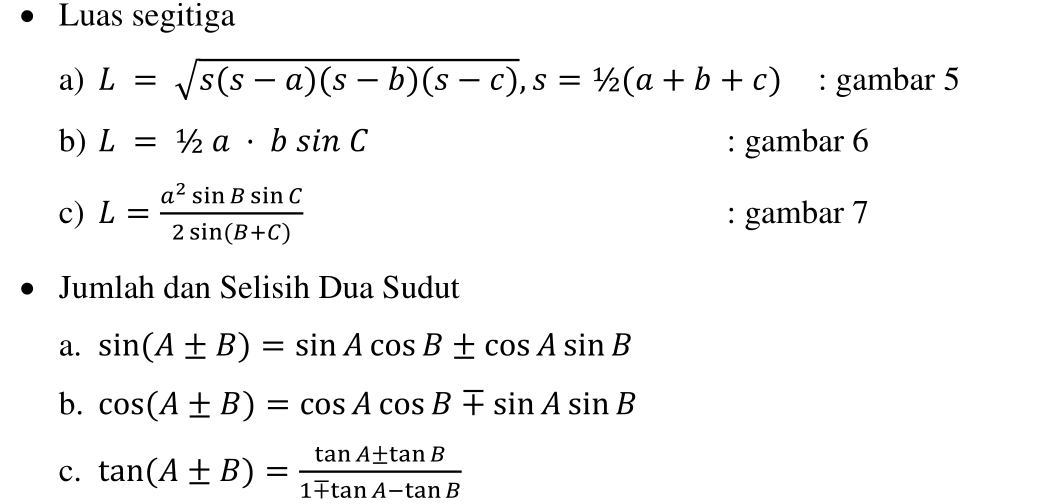
\includegraphics[width=0.9\linewidth]{pict/28}
		\end{center}
	\end{frame}

	\begin{frame}{Trigonometri}
		\begin{center}
			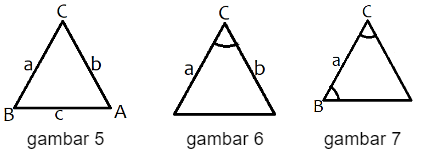
\includegraphics[width=0.5\linewidth]{pict/26}
			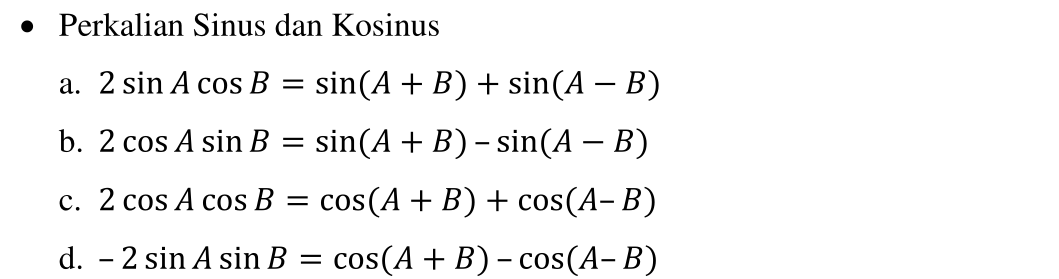
\includegraphics[width=0.9\linewidth]{pict/29}
		\end{center}
	\end{frame}

	\begin{frame}{Trigonometri}
		\begin{center}
			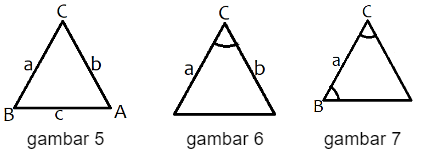
\includegraphics[width=0.5\linewidth]{pict/26}
			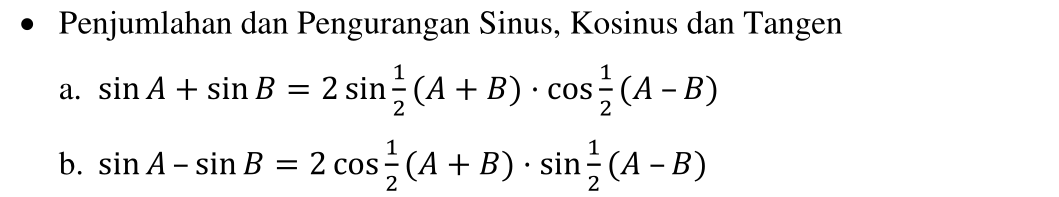
\includegraphics[width=0.9\linewidth]{pict/30}
			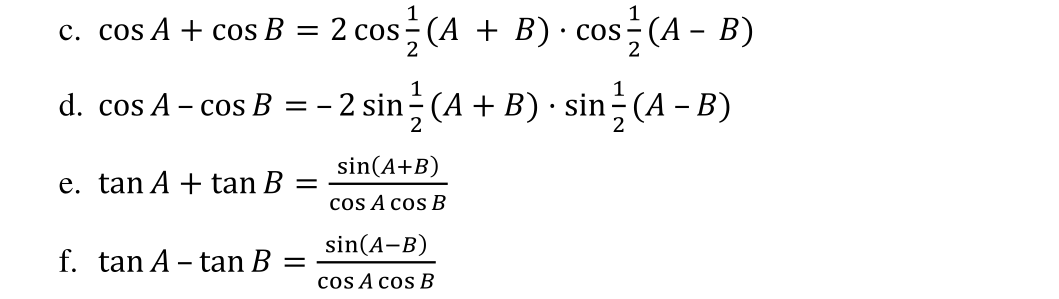
\includegraphics[width=0.9\linewidth]{pict/31}
		\end{center}
	\end{frame}

	\begin{frame}{Trigonometri}
		\begin{center}
			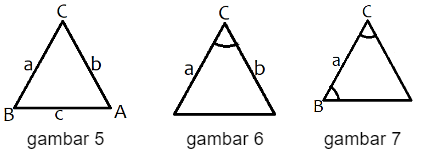
\includegraphics[width=0.5\linewidth]{pict/26}
			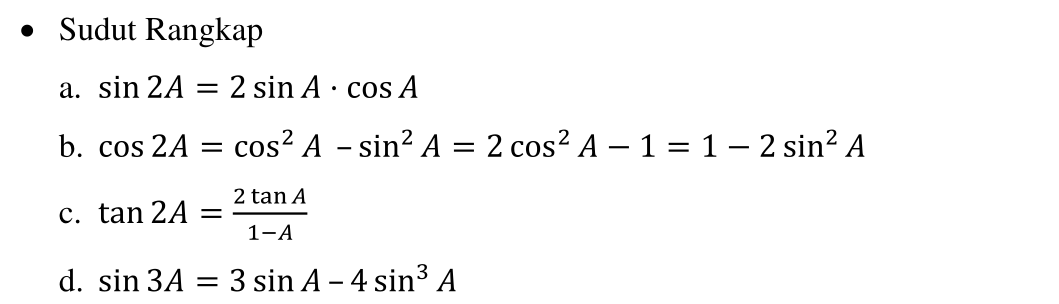
\includegraphics[width=0.9\linewidth]{pict/32}
		\end{center}
	\end{frame}

	\begin{frame}{Trigonometri}
		\begin{center}
			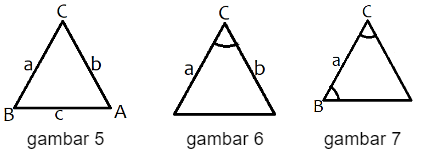
\includegraphics[width=0.5\linewidth]{pict/26}
			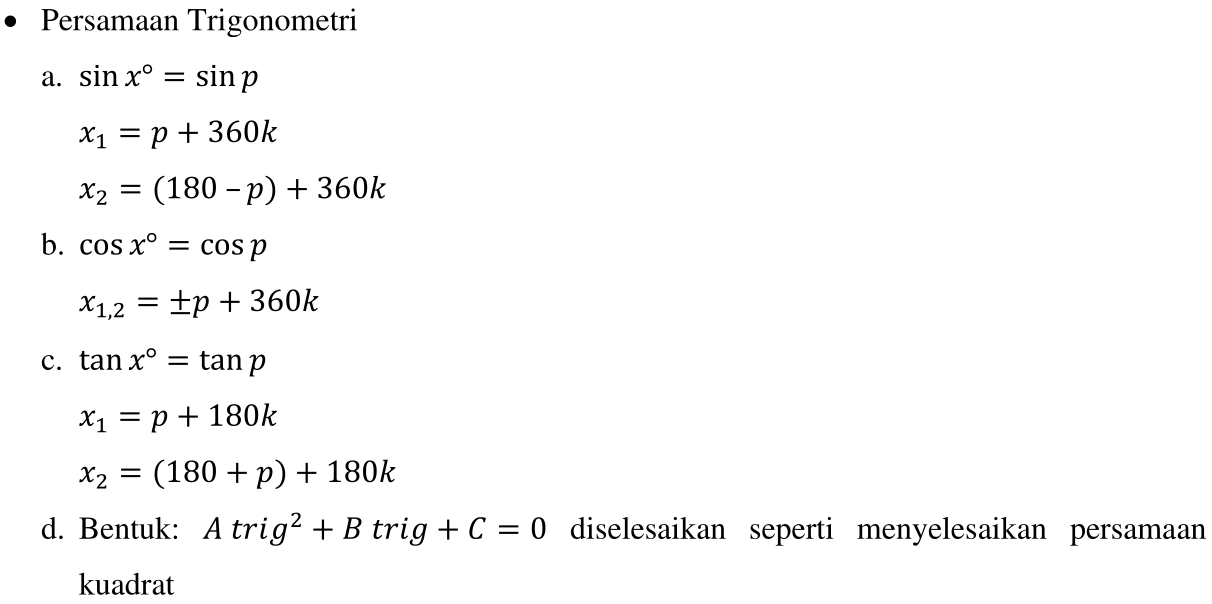
\includegraphics[width=0.9\linewidth]{pict/33}
		\end{center}
	\end{frame}

	\begin{frame}
		\frametitle{Soal Latihan}
		\begin{enumerate}
			\item Dalam suatu lingkaran yang berjari-jari 8 cm, dibuat segi-8 beraturan. Panjang sisi segi-8 tersebut adalah ... cm
			\item  Jika luas segi delapan beraturan adalah $ 200\sqrt{2}\text{ cm}^2 $ , maka panjang jari-jari lingkaran luarnya adalah ... cm
			\item Diketahui segitiga ABC dengan panjang sisi AB = 3 cm, AC = 4 cm, dan $ \angle $CAB = 60$ ^{\circ} $. CD adalah tinggi segitiga ABC. Panjang CD = ... cm
			\item Himpunan penyelesaian dari persamaan $ \cos(x + 210)^{\circ} + \cos(x - 210)^{\circ} = \frac{1}{2}\sqrt{3} $ untuk $ 0 \leq x \leq 360^{\circ} $ adalah ... 
			\item Pada segitiga ABC lancip, diketahui $ \cos A = \frac{4}{5} $ dan $ \sin B = \frac{12}{13} $, maka $ \sin C = \ldots $
		\end{enumerate}
	\end{frame}

\section{Turunan}

	\begin{frame}
		\frametitle{Turunan}
		Dimisalkan fungsi $ f $ terdefinisi pada selang terbuka $ I $ yang memuat $ c $. Turunan pertama dari fungsi $ f $ di titik $ c $ ditulis $ f'(c) $ didefinisikan sebagai:
		\begin{equation}
			f'(c) = \lim\limits_{x \rightarrow c} \frac{f(x) - f(c)}{x - c} ,
		\end{equation}
		jika limitnya ada.
	\end{frame}

	\begin{frame}{Turunan}
		Apabila dilakukan penggantian $ x = c + h $, jika $ x \rightarrow c \leftrightarrow h \rightarrow 0 $ dan $ x - c = h $, turunan fungsi $ f $ di $ c $ dapat dituliskan dalam bentuk:
		\begin{equation}
			f'(c) = \lim\limits_{h \rightarrow 0} \frac{f(c + h) - f(c)}{h}
		\end{equation}
	\end{frame}

	
	\begin{frame}{Turunan}
		\begin{itemize}
			\item Jika suatu fungsi konstan, misal $ f(x) = k $ untuk sembarang bilangan rill $ k $, maka
			\begin{equation}
				\frac{d}{dx}[k] = 0
			\end{equation}
			\item Jika $ n $ suatu bilangan bulat positif, maka:
			\begin{equation}
				\frac{d}{dx}[x^n] = n x^{n-1}
			\end{equation}
			\item Jika $ f $ fungsi yang dapat diturunkan di $ x $ dan $ k $ sebarang bilangan rill, maka $ kf $ juga dapat diturunkan di $ x $, yaitu:
			\begin{equation}
				\frac{d}{dx}[kf(x)] = k\frac{d}{dx}[f(x)]
			\end{equation}
		\end{itemize}
	\end{frame}

	\begin{frame}{Turunan}
		\begin{itemize}
			\item Jika $ f $ dan $ g $ fungsi yang dapat diturunkan di $ x $, maka $ f + g $ dan $ f - g $ juga dapat diturunkan di $ x $ dan
			\begin{equation}
				\frac{d}{dx}[f(x) + g(x)] = \frac{d}{dx}[f(x)] + \frac{d}{dx}[g(x)]
			\end{equation}
			\begin{equation}
				\frac{d}{dx}[f(x) - g(x)] = \frac{d}{dx}[f(x)] - \frac{d}{dx}[g(x)]
			\end{equation}
			\item Jika $ g $ dan $ g $ dapat diturunkan di $ x $, maka
			\begin{equation}
				\frac{d}{dx}[f(x)g(x)] = f(x)\frac{d}{dx}[g(x)] + \frac{d}{dx}[f(x)]g(x)
			\end{equation}
		\end{itemize}
	\end{frame}
	
	\begin{frame}{Turunan}
		\begin{itemize}
			\item Jika $ f $ dan $ g $ dua fungsi yang dapat diturunkan di $ x $, dan $ g(x) \neq 0 $ maka $ \frac{f}{g} $ juga dapat diturunkan di $ x $, dan
			\begin{equation}
				\frac{d}{dx}\left[ \frac{f(x)}{g(x)} \right] = \frac{\frac{d}{dx}[f(x)]g(x) + f(x)\frac{d}{dx}[g(x)]}{[g(x)]^2}
			\end{equation}
			\item Untuk turunan fungsi trigonometri sebagai berikut
			\begin{center}
				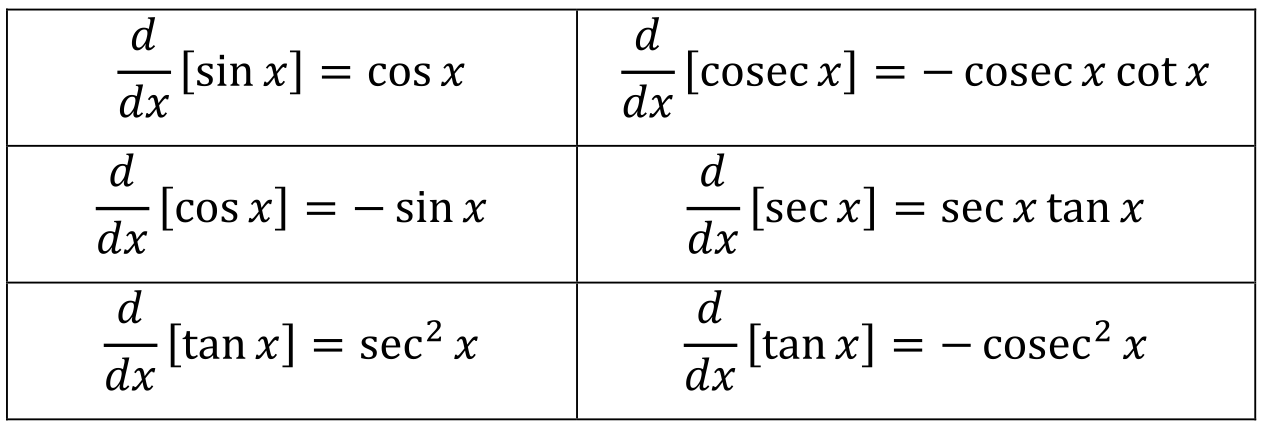
\includegraphics[width=0.7\linewidth]{pict/34}
			\end{center}
		\end{itemize}
	\end{frame}

	\begin{frame}
		\frametitle{Contoh 1}
		Menggunakan definisi turunan, tentukan turunan terhadap $ x $ dari $ f(x) = \sqrt{x} $
		\vfill\null
	\end{frame}

	\begin{frame}
		\frametitle{Contoh 2}
		Dapatkan turunan dari fungsi $ f(x) = 2x(x^2 + 1) $
		\vfill\null
	\end{frame}

	\begin{frame}
		\frametitle{Contoh 3}
		Dapatkan turunan dari fungsi $ f(x) = \sin5x $
		\vfill\null
	\end{frame}

	\begin{frame}
		\frametitle{Soal Latihan}
		\begin{enumerate}
			\item Carilah turunan fungsi berikut menggunakan definisi turunan
			\begin{enumerate}
				\item[a.] $ f(x) = x^2 + 5x $
				\item[a.] $ f(x) = \sqrt{x} + 1 $
				\item[c.] $ f(x) = \sin x $
			\end{enumerate}
			\item Tentukan $ f'(x) $ dan $ f'(1) $ jika
			\begin{enumerate}
				\item[a.] $ f(x) = \sqrt{5} $
				\item[b.] $ f(x) = 5\sqrt{x} $
				\item[c.] $ f(x) = \left(2x^2+5\right)^3 $
				\item[d.] $ f(x) = \frac{3x^3-5x}{x^2} $
				\item[e.] $ f(x) = x^2 \tan(2x+1) $
			\end{enumerate}
		\vfill\null
		\end{enumerate}
	\end{frame}

\section{Integral}
	
	\subsection{Integral Tak Tentu}
		
		\begin{frame}
			\frametitle{Integral Tak Tentu}
		\end{frame}
	
	\subsection{Integral dengan Substitusi}
	
		\begin{frame}
			\frametitle{Integral dengan Substitusi}
		\end{frame}
	
	\subsection{Integral Tentu}
	
		\begin{frame}
			\frametitle{Integral Tentu}
		\end{frame}

\end{document}
